%%%%%%%%%%%%%%%%%%%%%%%%%%%%%%%%%%%%%%%%%%%%%%%%%%%%%%%%%%%%%%%%%%%%%%%%%%%%%%%
%% SOCIOL 723 -- Social Statistics II
%% Week 14 -- Synthesis and Exam Review
%% Wenhao Jiang, Duke University, Fall 2026
%%%%%%%%%%%%%%%%%%%%%%%%%%%%%%%%%%%%%%%%%%%%%%%%%%%%%%%%%%%%%%%%%%%%%%%%%%%%%%%

\documentclass[aspectratio=169,11pt,xcolor=dvipsnames]{beamer}
\mode<presentation>

%% ---- fonts: Latin Modern Roman (the LaTeX default), serif throughout -------
\usepackage[T1]{fontenc}
\usepackage{lmodern}
\usefonttheme{serif}
\renewcommand{\familydefault}{\rmdefault}

%% ---- packages --------------------------------------------------------------
\usepackage{amsmath,amsfonts,amssymb,bm}
\usepackage{graphicx}
\usepackage{booktabs}
\usepackage{tikz}
\usetikzlibrary{arrows.meta,positioning,calc}
\usepackage[english]{babel}

\newcommand{\srcp}[1]{{\scriptsize\color{gray}(#1)}}
\newcommand{\srct}[1]{#1}

\DeclareMathOperator*{\argminop}{arg\,min}
\DeclareMathOperator*{\argmaxop}{arg\,max}
%% \limits forces the subscript underneath even in inline math
\newcommand{\argmin}{\argminop\limits}
\newcommand{\argmax}{\argmaxop\limits}
\DeclareMathOperator{\Cov}{Cov}
\DeclareMathOperator{\Var}{Var}
\DeclareMathOperator{\trace}{tr}
\DeclareMathOperator{\rank}{rank}
\DeclareMathOperator{\plim}{plim}
\newcommand{\indep}{\perp\!\!\!\perp}

%% ---- notation conventions (course-wide) ------------------------------------
\newcommand{\E}{E}
\newcommand{\En}{\mathbb{E}_n}
\newcommand{\R}{\mathbb{R}}
\newcommand{\X}{\bm{X}}
\newcommand{\Y}{\bm{y}}
\newcommand{\Ix}{\bm{I}}
\newcommand{\zero}{\bm{0}}
\newcommand{\bhat}{\hat{\bm{\beta}}}
\newcommand{\dto}{\overset{d}{\longrightarrow}}
\newcommand{\pto}{\overset{p}{\longrightarrow}}
\usetikzlibrary{shapes,decorations.pathmorphing}
\newcommand{\lik}{\mathcal{L}}
\newcommand{\loglik}{\ell}
\newcommand{\Info}{\mathcal{I}}
\newcommand{\SE}{\mathrm{se}}

%% ---- theme -----------------------------------------------------------------
\usetheme{default}
%% thin single-line header: clickable section names, current one highlighted.
%% (miniframes is deliberately not used: one dot per slide wraps to 4 rows here)
\setbeamerfont{section in head/foot}{size=\tiny}
\setbeamertemplate{headline}{%
  \begin{beamercolorbox}[wd=\paperwidth,ht=2.4ex,dp=1.1ex,%
                         leftskip=.3cm,rightskip=.3cm]{section in head/foot}%
    \usebeamerfont{section in head/foot}%
    \insertsectionnavigationhorizontal{.94\paperwidth}{}{}%
  \end{beamercolorbox}%
}

\definecolor{dukeblue}{RGB}{1,33,105}
\definecolor{accent}{RGB}{200,78,0}
\definecolor{softgray}{RGB}{242,242,245}

\setbeamercolor{structure}{fg=dukeblue}
\setbeamercolor{frametitle}{fg=dukeblue,bg=white}
\setbeamercolor{section in head/foot}{fg=white,bg=dukeblue}
\setbeamercolor{section in head/foot shaded}{fg=white!50!dukeblue,bg=dukeblue}
\setbeamercolor{alerted text}{fg=accent}
\setbeamercolor{block title}{fg=white,bg=dukeblue}
\setbeamercolor{block body}{fg=black,bg=softgray}
\setbeamercolor{block title alerted}{fg=white,bg=accent}
\setbeamercolor{block body alerted}{fg=black,bg=softgray}

\setbeamertemplate{footline}[page number]
\setbeamertemplate{navigation symbols}{}
%% continued frames keep the SAME font size and spill onto a new slide
\setbeamertemplate{frametitle continuation}{\normalfont\footnotesize\ (cont.)}
\setbeamertemplate{itemize items}[circle]
\setbeamertemplate{blocks}[rounded][shadow=false]
\setbeamerfont{frametitle}{series=\bfseries}
\setbeamerfont{footnote}{size=\scriptsize}
\setbeamerfont{caption}{size=\footnotesize}
\setbeamertemplate{subsection in head/foot}{}
\setbeamertemplate{subsection in head/foot shaded}{}
\setbeamertemplate{caption}[numbered]

\newcommand{\adv}{\,\raisebox{0.6pt}{\textcolor{accent}{$\bigstar$}}}

\setbeamertemplate{section page}{%
  \begin{centering}\vfill
  {\usebeamercolor[fg]{structure}\Large\bfseries\insertsectionhead\par}
  \vskip4pt{\color{dukeblue}\rule{0.35\linewidth}{1pt}\par}
  \vfill\end{centering}}
\setbeamertemplate{subsection page}{%
  \begin{centering}\vfill
  {\usebeamercolor[fg]{structure}\large\bfseries\insertsubsectionhead\par}
  \vfill\end{centering}}

\AtBeginDocument{%
  \setlength{\abovedisplayskip}{5pt}%
  \setlength{\belowdisplayskip}{5pt}%
  \setlength{\abovedisplayshortskip}{2pt}%
  \setlength{\belowdisplayshortskip}{3pt}%
}
\setbeamertemplate{frametitle}{%
  \vskip4pt\usebeamerfont{frametitle}\usebeamercolor[fg]{frametitle}%
  \insertframetitle\par\vskip2pt}
\setbeamersize{text margin left=0.75cm, text margin right=0.75cm}

%% ---- title -----------------------------------------------------------------
\title[SOCIOL 723]{SOCIOL 723: Social Statistics II\\[2pt]}
\subtitle{\large Week 14, Synthesis and Exam Review\\[-8pt]}
\author[Jiang]{\large Wenhao Jiang\vspace{-1.5em}}
\institute[Duke]{}
\titlegraphic{
\includegraphics[height=1.3cm]{../Misc/duke_logo.png}}
\date{\large Department of Sociology, Fall 2026}


\begin{document}

\begin{frame}[plain]
  \titlepage
\end{frame}

\begin{frame}{Today}
\begin{itemize}\itemsep6pt
  \item A synthesis: what the semester was actually about.
  \item A decision guide you can use on your own data.
  \item The final exam: what it covers, how it is run, and how to prepare.
\end{itemize}
\vskip8pt
\begin{block}{Logistics}
No lab Thursday November 26 (Thanksgiving recess). \\
\textbf{Cumulative final exam} in the December examination period.
\end{block}
\end{frame}

%%%%%%%%%%%%%%%%%%%%%%%%%%%%%%%%%%%%%%%%%%%%%%%%%%%%%%%%%%%%%%%%%%%%%%%%%%%%%%%
\section[Synthesis]{What the Semester Was About}
%%%%%%%%%%%%%%%%%%%%%%%%%%%%%%%%%%%%%%%%%%%%%%%%%%%%%%%%%%%%%%%%%%%%%%%%%%%%%%%
\begin{frame}\sectionpage\end{frame}

\begin{frame}{Three Questions, in Order}
\begin{enumerate}\itemsep5pt
  \item \textbf{What am I trying to estimate?} A unit-specific quantity and a
        target population. ATE, ATT, LATE, the effect at a cutoff, $\tau(x)$.
        Weeks 5 and 13.
  \item \textbf{What would have to be true for my estimate to recover it?}
        Ignorability, exclusion, continuity, parallel trends. Weeks 5--11.
  \item \textbf{How do I estimate it, and how uncertain am I?} Least squares,
        maximum likelihood, weighting, orthogonal scores, cross-fitting. Weeks
        1--4, 6, 12--13.
\end{enumerate}
\vskip6pt
\begin{alertblock}{The ordering is the lesson}
Most quantitative papers start at 3 and never articulate 1 or 2. Most
methodological disputes are really disagreements at 1 or 2 being conducted as if
they were about 3.
\end{alertblock}
\end{frame}

\begin{frame}{One Idea, Recurring}
\begin{center}
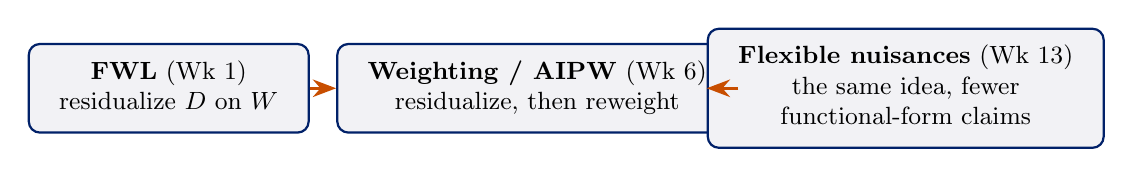
\begin{tikzpicture}[scale=0.9,>=Stealth,thick,font=\small]
  \node[draw=dukeblue,rounded corners,inner sep=5pt,fill=softgray] (a) at (0,0)
    {\begin{tabular}{c}\textbf{FWL} (Wk 1)\\ residualize $D$ on $W$\end{tabular}};
  \node[draw=dukeblue,rounded corners,inner sep=5pt,fill=softgray] (b) at (5.2,0)
    {\begin{tabular}{c}\textbf{Weighting / AIPW} (Wk 6)\\ residualize, then reweight\end{tabular}};
  \node[draw=dukeblue,rounded corners,inner sep=5pt,fill=softgray] (c) at (10.4,0)
    {\begin{tabular}{c}\textbf{Flexible nuisances} (Wk 13)\\ the same idea, fewer\\ functional-form claims\end{tabular}};
  \draw[->,accent,very thick] (a)--(b); \draw[->,accent,very thick] (b)--(c);
\end{tikzpicture}
\end{center}
\vskip4pt
\begin{itemize}\itemsep3pt
  \item \textbf{Partialling out} is the through-line. Remove the part of the
        treatment explained by the controls; use what is left.
  \item Its virtue is \emph{insensitivity}: small errors in how you model the
        controls do not contaminate the parameter you care about.
  \item Everything else, matching, weighting, IV, RD, DID, synthetic control
, is a different answer to the question \emph{where does the
        counterfactual come from?}
\end{itemize}
\end{frame}

\begin{frame}[allowframebreaks,t]{Every Design, in One Table}
\begin{center}\footnotesize
\renewcommand{\arraystretch}{1.25}
\begin{tabular}{llll}
\toprule
Design & Key assumption & Estimand & Main threat \\
\midrule
Regression / matching / IPW & ignorability given $X$ & ATE, ATT, ATO & unmeasured confounding \\
AIPW / DML & ignorability $+$ rates & ATE, $\tau(x)$ & same, ML does not identify \\
IV / 2SLS & relevance, independence, exclusion, monotonicity & LATE (compliers) & weak or invalid instrument \\
RD (sharp) & continuity at $c$ & effect at the cutoff & manipulation; bandwidth \\
RD (fuzzy) & $+$ first-stage jump, monotonicity, exclusion & compliers at the cutoff & weak first stage \\
DID (2$\times$2) & parallel trends, no anticipation & ATT & differential trends \\
DID, staggered & cohort-wise parallel trends vs.\ not-yet-treated, no anticipation & ATT$(g,t)$, then aggregate & TWFE contamination \\
Synthetic control & factor model, long pre-period & ATT for one unit & poor pre-fit; interpolation \\
\bottomrule
\end{tabular}
\end{center}
\vskip5pt
\begin{itemize}\itemsep2pt
  \item \alert{No row is safer than the others in the abstract.} Credibility is a
        property of the application, not of the method.
  \item Notice how often the estimand is chosen \emph{by the design} rather than
        by the researcher. Say so when it is.
\end{itemize}
\end{frame}

\begin{frame}[allowframebreaks,t]{Inference, in One Table}
\begin{center}\footnotesize
\renewcommand{\arraystretch}{1.25}
\begin{tabular}{lll}
\toprule
Situation & Use & Week \\
\midrule
Default & HC2 or HC3 robust & 2 \\
Treatment assigned in groups & cluster on the assignment level & 2 \\
Fewer than $\sim$40 clusters & CR2 $+$ Satterthwaite, or wild cluster bootstrap & 2 \\
Nonlinear quantity of interest & delta method, simulation, or bootstrap & 2, 4 \\
Nuisance function estimated & bootstrap the whole pipeline, or an influence function & 6 \\
Weak instrument & Anderson--Rubin & 7 \\
One treated unit & permutation / placebo inference & 11 \\
ML nuisances & orthogonal score $+$ cross-fitting & 13 \\
\bottomrule
\end{tabular}
\end{center}
\vskip5pt
\alert{The recurring error is a standard error that ignores a step in the
procedure}, estimated weights, a selected model, a matched design, a chosen
bandwidth. When in doubt, bootstrap the whole pipeline, resampling in a way that
\emph{reproduces the sampling or assignment structure} (clusters as clusters,
panels as panels). But the bootstrap is not universal: it is \emph{invalid} for
nearest-neighbour matching (Week 6), and unreliable more generally for
non-smooth, boundary, post-selection, and weakly identified procedures.
\end{frame}

\begin{frame}{A Decision Guide}
\begin{enumerate}\itemsep3pt
  \item Write the theoretical estimand in one sentence: unit-specific quantity,
        target population.
  \item Draw the DAG. Mark what is unobserved.
  \item Ask: \emph{is there any set I can measure that closes the back doors?}
  \begin{itemize}\itemsep1pt
    \item Yes $\to$ selection on observables. Check overlap, use a doubly robust
          estimator, report a sensitivity analysis (Week 6).
    \item No $\to$ look for design-based variation: an instrument (7), a threshold
          (9), a policy change over time (10), a single treated unit with a long
          pre-period (11).
  \end{itemize}
  \item Check whether the design's estimand is the one you wrote in step 1. If
        not, say so explicitly rather than quietly redefining the question.
  \item Choose inference to match the design.
  \item If $W$ is high-dimensional or the functional form is a guess, use an
        orthogonal score with cross-fitting (13).
  \item Report what would change your mind.
\end{enumerate}
\end{frame}

\begin{frame}{Things That Are Never a Solution}
\begin{itemize}\itemsep3pt
  \item \alert{Adding more controls} without a DAG. Bad controls exist, and
        ``kitchen sink'' amplifies bias as often as it reduces it (Week 5).
  \item \alert{Robust standard errors} for a problem of bias (Week 2).
  \item \alert{A high $R^2$}, or a high AUC, as evidence of causality (Weeks 1,
        12).
  \item \alert{A non-significant specification test}, balance $t$-tests,
        Sargan, pre-trend tests, as evidence that an assumption holds. Low
        power is not confirmation (Weeks 6, 7, 10).
  \item \alert{Machine learning} for an identification problem (Week 13).
  \item \alert{Reporting whichever specification worked.} Pre-commit, then show
        robustness.
\end{itemize}
\vskip3pt
Each of these is a real move made in published sociology, and you now have the
vocabulary to say precisely why it fails.
\end{frame}

%%%%%%%%%%%%%%%%%%%%%%%%%%%%%%%%%%%%%%%%%%%%%%%%%%%%%%%%%%%%%%%%%%%%%%%%%%%%%%%
\section[Final Exam]{The Final Exam}
%%%%%%%%%%%%%%%%%%%%%%%%%%%%%%%%%%%%%%%%%%%%%%%%%%%%%%%%%%%%%%%%%%%%%%%%%%%%%%%
\begin{frame}\sectionpage\end{frame}

\begin{frame}{What the Exam Covers}
Cumulative, but \alert{weighted towards Weeks 9--13}: the midterm already
examined Weeks 1--7, and this is the only assessment that reaches the second
half of the course.
\vskip4pt
\begin{itemize}\itemsep3pt
  \item \textbf{Everything developed in scalar form is examinable.} Frames marked
        \adv{} are not: matrix derivations, projection geometry, asymptotic
        arguments.
  \item For every design, you should be able to state \emph{what it assumes},
        \emph{what it estimates}, and \emph{how it fails}. That is the table from
        earlier today, and it is the spine of the exam.
  \item Expect to read a short description of a study and say which design it is,
        what its estimand is, and what you would need to believe.
  \item No code. You may be asked to interpret \texttt{R} output.
\end{itemize}
\end{frame}

\begin{frame}{Format and Rules}
\begin{block}{Logistics}
Held in the University examination period in December; the Registrar sets the
date and time. Open book and open note, but \textbf{timed}.
\end{block}
\vskip5pt
\begin{alertblock}{No AI}
Unlike the problem sets, no AI assistance of any kind. This is deliberate. It is
the one place in the course where what is being assessed is unambiguously
\emph{your} understanding rather than what a tool can produce for you.
\end{alertblock}
\vskip5pt
Bring the slides and your own notes. Notes you wrote yourself are far more useful
under time pressure than a printout you have never read.
\end{frame}

\begin{frame}{How to Prepare}
\begin{enumerate}\itemsep4pt
  \item \textbf{Work the checkpoints.} Each deck has a ``what you should be able
        to do'' frame. If you can do those without notes, you are ready.
  \item \textbf{Rebuild the four tables} from today: design, assumption, estimand,
        threat; and the inference table. Write them from memory, then check.
  \item \textbf{Re-derive the short results by hand}: the normal equations, the
        scalar variance, omitted-variable bias, the Wald ratio, the $2\times2$
        DID. None takes more than a few lines.
  \item \textbf{Re-read your own problem sets}, especially anything you got wrong.
        That is the highest-yield hour you can spend.
\end{enumerate}
\vskip5pt
\alert{The exam rewards judgement, not recall.} If you can say why a design is
the wrong one for a question, you understand it.
\end{frame}

\begin{frame}[allowframebreaks,t]{Where to Go Next}
\begin{itemize}\itemsep3pt
  \item \textbf{Depth on design}: Angrist and Pischke, \textit{Mostly Harmless
        Econometrics}; Cunningham, \textit{Causal Inference: The Mixtape};
        Huntington-Klein, \textit{The Effect}.
  \item \textbf{Depth on potential outcomes}: Imbens and Rubin,
        \textit{Causal Inference for Statistics, Social, and Biomedical Sciences};
        Morgan and Winship.
  \item \textbf{Depth on graphs}: Pearl, \textit{Causality}; Hern\'an and Robins,
        \textit{Causal Inference: What If}.
  \item \textbf{Depth on causal ML}: Chernozhukov et al., \textit{Applied Causal
        Inference Powered by ML and AI}.
  \item \textbf{In this department}: measurement and latent variables,
        computational text analysis, network methods, demographic methods,
        multilevel models, each of which assumes what you now know.
\end{itemize}
\vskip4pt
\begin{alertblock}{The one thing to keep}
Say what you are estimating, say what would have to be true, and say what would
change your mind. Everything else is technique.
\end{alertblock}
\end{frame}

\end{document}
